\documentclass[a4paper]{scrbook}
\usepackage[utf8]{inputenc}
\usepackage[ngerman]{babel}

\usepackage{array}            % Tabellen im Mathemodus (Matrizen)
\usepackage{graphicx}         % Einbindung von Grafiken
\usepackage{braket}           % ermöglicht die Verwendung von Diracs Bra-Ket-Notation
\usepackage{esdiff}           % für Ableitungen

\usepackage{hyperref}         % für automatische Verlinkungen in der pdf
\usepackage{datatool}	      % muss verwendet werden, da glossaries sonst einen Fehler verursacht
\usepackage[toc]{glossaries}  % Glossar

\makeglossaries
\makeindex

% Glossar
\newglossaryentry{OST}{name={OST}, description={Opposite Side Tagger}}
\newglossaryentry{Toy MC}{name={Toy MC}, description={Zur Validierung des Fitters werden zufällig Daten gemäß einer gewünschten Verteilung generiert und im Anschluss gefittet}}


% Definiere Kürzel
\newcommand{\SJPsi}{S_{J/\Psi K_s^0}}


\begin{document}

% Binde Titelseite ein
\begin{titlepage}
\begin{center}
 
\Large\textbf{Fakultät für Physik und Astronomie\\
Ruprecht-Karls-Universität Heidelberg}

\vspace{17cm}

\normalsize
Bachelorarbeit in Physik\\
eingereicht von\\
\vspace{0.5cm}
\Large\textbf{Patrick Fahner}\\
\normalsize
\vspace{0.5cm}
geboren in Mannheim (Deutschland)\\
\vspace{0.5cm}
\Large\textbf{August 2013}
\normalsize

\newpage




\Large\textbf{About ...}

\vspace{18cm}

\normalsize
This Bachelor Thesis has been carried out by XYZ at the\\
ABC Institute in Heidelberg\\
under the supervision of\\
Prof. Max Mustermann

\vfill
\end{center}

\end{titlepage}



\chapter{CP-Verletzung in B-Meson-Systemen}
\section{Diskrete Symmetrietransformationen}
Symmetrien sind in der Physik von zentraler Bedeutung. Gemäß dem Noether-Theorem existiert in der klassischen Physik zu jeder kontinuierlichen Symmetrie eine Erhaltungsgröße. In quantenmechanischen Systemen können wir drei diskrete Symmetrietransformationen betrachten:
\begin{enumerate}
\item \textbf{Parität $\mathcal{P}$:} \\
      Bei der Paritätsoperation wird das Vorzeichen der kartesischen Ortskoordinaten umgekehrt. Dies entspricht einer Punktspigelung.
\item \textbf{Ladungskonjugation $\mathcal{C}$:} \\
      Jedes Teilchen wird durch sein Antiteilchen ersetzt.
\item \textbf{Zeitumkehr $\mathcal{T}$:} \\
      Das Vorzeichen auf der Zeitachse wird umgekehrt. Da in der vorligenden Arbeit allerdings nur die CP-Verletzung gemessen werden soll, wird die Zeitumkehr im folgenden vernachlässigt.
\end{enumerate}
Entgegen der klassischen Intuition konnte Wu 1956 nachweisen, dass die Parität im $\beta$-Zerfall und damit in der schwachen Wechselwirkung nicht erhalten ist. Weitere Experimente zeigen, dass die schwache Wechselwirkung die Parität maximal verletzt: Neutrinos, die nur schwach wechselwirken können, sind stets \glqq linkshändig\grqq (Spin und Impuls antiparallel), Antineutrinos dagegen immer \glqq rechtshändig\grqq (Spin und Impuls parallel). Da der Spin im Gegensatz zum Impuls invariant unter $\mathcal{P}$-Transformation ist, würde diese Operation aus einem linkshändigen Neutrino ein rechtshändiges machen, was in der Nautr nicht realisiert ist.

Damit ist offensichtlich, dass die schwache Wechselwirkung auch die Ladungskonjugation verletzt: Wendet man die $\mathcal{C}$-Transformation auf ein linkshändiges Neutrino an, so erhält man ein linkshändiges Antineutrino. Dieses existiert aber wie bereits erwähnt nicht. Analog gilt die Überlegung auch für Antineutrinos.

\subsection{Scheinbare $\mathcal{CP}$-Invarianz}
Wendet man nun aber die Transformationen $\mathcal{P}$ und $\mathcal{C}$ direkt hintereinander an, so ergibt sich zunächst kein Widerspruch zur Natur (siehe Abb. \ref{fig:cp_invaranz}). Aus einen linkshändigen Neutrino wird ein rechtshändiges Antineutrino. Im Jahre 1964 wurde dann allerdings im Zerfall neutraler K-Mesonen erstmal $\mathcal{CP}$-Verletzung nachgewiesen. \cite{kleinknecht}

\begin{figure}[hptb]
\centering
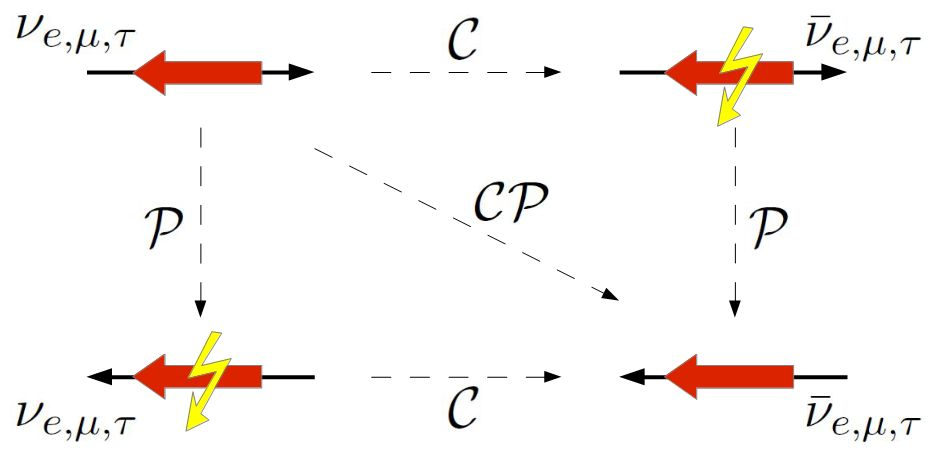
\includegraphics[width = 0.8\textwidth]{cp_invarianz}
\caption{Scheinbare $\mathcal{CP}$-Invarianz: Während eine reine $\mathcal{P}$- oder $\mathcal{C}$-Transformation zu in der Natur nicht realisierten Zuständen führt, scheint es bei der kombinierten $\mathcal{CP}$-Transformation keinen Widerspruch zu geben (dünne Pfeile: Impulsausrichtung, dicke Pfeile: Spinausrichtung).}
\label{fig:cp_invarianz}
\end{figure}

\section{Mischung im B-Mesonen-System}
Die Flavoureigenzustände $\Bra{B^0} = \Bra{\bar{b}d}$ und $\Bra{\bar{B^0}} = \Bra{b\bar{d}}$ entsprechen nicht den Masseneigenzuständen. Wir definieren daher die normierten Zustände
\begin{align}
\Bra{B_h} = p \Bra{B^0} - q \Bra{\bar{B^0}} \label{eq:b_heavy}\\ 
\Bra{B_l} = p \Bra{B^0} + q \Bra{\bar{B^0}} \label{eq:b_light}\\
\text{mit} \quad |p|^2 + |q|^2 = 1
\end{align}
welche eine definierte Masse und Zerfallsbreite besitzen. Sie sind auch Eigenzustände eines nicht-hermiteschen Hamiltonoperators (Nichthermitizität wegen des möglichen Zerfalls der Teilchens). Dieser setzt sich zusammen aus den hermiteschen Massenoperatoren $M$ und $\Gamma$. Notieren wir die lineare Superposition der Zustände \ref{eq:b_heavy} und \ref{eq:b_light} als $\begin{pmatrix} p \\ q \end{pmatrix}, so nimmt die zeitabhängige Schrödingergleichung die Form
\begin{align}
\imath \diff{}{t}\begin{pmatrix} p \\ q \end{pmatrix} = \left(M - \frac{\imath}{2} \Gamma\right) \begin{pmatrix} p \\ q \end{pmatrix}
\end{align}
an und führt zur folgenden zeitlichen Entwicklung der Zustände:
\begin{align}

\end{align}


\chapter{Abschätzung systematischer Fehler}
\section{Tagging Kalibrierung}
Im Fit wird bei den Parametern der Tagging Kalibrierung nur der statistischen Fehler berücksichtigt. Es soll nun an dieser Stelle der Einfluss der statistischen Unsicherheiten abgeschätzt werden. \\
Die Korrekturparameter $p_0$ und $p_1$ für die Fehlerwahrscheinlichkeit des \gls{OST} sind gegeben durch
\begin{align}
p_0 &= 0,392 \pm 0,0017\ \text{(stat.)} \pm 0,0076\ \text{(syst.)} \\
p_1 &= 1,035 \pm 0,021\ \text{(stat.)} \pm 0,0076\ \text{(syst.)}.
\end{align}

\paragraph{Variation der Parameter in den Daten}
Zunächst werden die Startwerte der Parameter $p_0$ und $p_1$ variiert, indem man jeweils den systematischen Fehler der Parameter addiert bzw. subtrahiert und dann den Fit auf die Daten durchührt. Für alle vier Kombinationen wird dann die Abweichung vom regulären Fitergebnis für $\SJPsi$ berechnet. Der Referenzwert aus dem Fit beträgt
\begin{align}
\SJPsi = 0,625 \pm 0,069
\end{align}

\begin{table}[hptb]
\centering
\caption{Variation des Fitergebnisses für $\SJPsi$ bei Veränderung der Startwerte für $p_0$ und $p_1$ $\pm$ ihrer statistischen Unsicherheiten}
\label{tab:syst_fit_calib_data}
$\begin{array}{cc|c|c}
\hline\hline
p_0            & p_1           & \SJPsi          & \Delta\SJPsi   \\ \hline
0,392 - 0,0076 & 1,035 - 0,012 & 0,599 \pm 0,067 & -0,026 \pm xxx \\
0,392 + 0,0076 & 1,035 - 0,012 & 0,661 \pm 0,072 & 0,036 \pm xxx \\
0,392 - 0,0076 & 1,035 + 0,012 & 0,592 \pm 0,066 & -0,033 \pm xxx \\
0,392 + 0,0076 & 1,035 + 0,012 & 0,651 \pm 0,071 & 0,026 \pm xxx \\
\hline\hline
\end{array}$
\end{table}

Die Ergebnisse sind Tabelle \ref{tab:syst_fit_calib_data} zu entnehmen. Die größte Abweichung beträgt hier $\Delta\SJPsi = 0,036$.

\paragraph{Variation der Parameter in \gls{Toy MC}}
Eine weitere Möglichkeit der Abschätzung besteht darin, sich entsprechende Toys zu generieren und diese dann zu fitten. Im Folgenden werden bei der Toy Generierung die Parameter $p_0$ und $p_1$ um ihre systematische Unsicherheiten variiert, der Fit dann allerdings mit den ursprünglichen Parameterwerten durchgeführt. Als Referenzwert generieren und fitten wir toys mit den ursprünglichen Parameterwerten $p_0$ und $p_1$ sowie $\SJPsi = 0.75$ und erhalten hierfür:

\begin{align}
\SJPsi = 0,75527 \pm xxx
\end{align}

\begin{table}[hptb]
\centering
\caption{Variation des Fitergebnisses für $\SJPsi$ bei Veränderung der Parameterwerte $p_0$ und $p_1$ $\pm$ ihrer statistischen Unsicherheiten bei der Generierung von Toys}
\label{tab:syst_fit_calib_toys}
$\begin{array}{cc|c|c}
\hline\hline
p_0            & p_1           & \SJPsi          & \Delta\SJPsi   \\ \hline
0,392 - 0,0076 & 1,035 - 0,012 & 0,782 \pm xxx & 0,027 \pm xxx \\
0,392 + 0,0076 & 1,035 - 0,012 & 0,719 \pm xxx & -0,036 \pm xxx \\
0,392 - 0,0076 & 1,035 + 0,012 & 0,788 \pm xxx & 0,032 \pm xxx \\
0,392 + 0,0076 & 1,035 + 0,012 & 0,727 \pm xxx & -0,028 \pm xxx \\
\hline\hline
\end{array}$
\end{table}

Die Ergebnisse sind Tabelle \ref{tab:syst_fit_calib_toys} zu entnehmen. Die größte Abweichung beträgt hier betragsmäßig ebenfalls $\Delta\SJPsi = 0,036$. Daher schätzen wir den systematischen Fehler durch die Tagging Kalibrierung auf 

\begin{align}
s_{tag_calib} = 0.036 \ .
\end{align}

\begin{thebibliography}{---}
\bibitem{kleinknecht}  K. Kleinknecht, Uncovering ...
\end{thebibliography}

\printglossaries 
% Selbstständigkeitserklärung
\chapter*{Erklärung}

Ich versichere, dass ich diese Arbeit selbstständig verfasst und keine anderen als die angegebenen Quellen und Hilfsmittel benutzt habe. \\
\vspace{0.2cm}
\begin{flushleft}
Heidelberg, den 19.08.2013,\\
\vspace{2cm}
%Unterschrift
Patrick Fahner
\end{flushleft}


\end{document}


